\providecommand{\main}{..}
\documentclass[\main/main.tex]{subfiles}
\begin{document}

\chapter{Struttura del tema d'esame}

Un tema d'esame di Ricerca Operativa risulta composto da 4/5 esercizi pratici e talvolta alcune domande di teoria.

Gli argomenti più frequenti negli esercizi sono, in ordine, i seguenti:

\begin{enumerate}
  \item Risolvere graficamento un problema di programmazione lineare. Si evidenzi il vertice ottimo e si riporti il valore di z per tutte le variabili del modello, compreso scarto e surplus. [12]
  \item Risolvere mediante scarti complementari la soluzione duale del problema. [11]
  \item Formulare un modello di Programmazione Lineare [11]
  \item Applicare Algoritmo di Ford-Fulkerson [10]
  \item Risolvere per via grafica valori per cui la composizione della base ottima non cambia. [9]
  \item Trovare un taglio di capacità minima [8]
  \item Branch \& Bound, Problema dello zaino [7]
  \item Taglio di Gomory relativo al primo vincolo del PL. [6]
  \item Si costruisca un reinstradamento che vada a ridurre il costo (o se ci si trova in condizione di minimo, di aumentarlo) modificandolo solo una volta e fornire la variazione di costo così ottenuta. [6]
  \item Forma canonica del Tableau [4]
  \item Determinare e disegnare il flusso massimo di un grafo [4]
\end{enumerate}

Seguono le tipologie di esercizi.

\section{Primo esercizio (8 punti)}

\subsection{Problema di Programmazione Lineare}
\begin{enumerate}
  \item Disegnare la regione ammissibile dai vincoli forniti. Si evidenzi il vertice ottimo e si riporti il valore di z per tutte le variabili del modello, compreso scarto e surplus. [12]
  \item Vi sono vertici ammissibili ai quali corrispondono basi degeneri?
  \item Risolvere per via grafica valori per cui la composizione della base ottima non cambia. [9]
  \item Da quali variabili è composta la base associata al vertice di una data intersezione?[2]
  \item Quanto può variare il termine noto senza che la composizione della base ottima cambi?
  \item Risolvere mediante scarti complementari la soluzione duale del problema. [11]
\end{enumerate}

\subsection{Problema di Programmazione Lineare Grafico}
\begin{enumerate}
  \item Verso dei vincoli rappresentati graficamente.
  \item Risolvere per via grafica valori per cui la composizione della base ottima non cambia.
\end{enumerate}


\section{Secondo esercizio}

\subsection{Problema di Minimo con Tableau [3]}

\begin{enumerate}
  \item Forma canonica del Tableau [4]
  \item Per quale dei valori rimanenti il Tableau corrisponde a:
        \begin{enumerate}
          \item Valori per ottimo finito [3]
          \item Soluzione non ottima e degenere [3]
          \item Problema illimitato [3]
        \end{enumerate}
  \item Disegnare la regione ammissibile al rilassamento continuo del problema. [2]
  \item Individuare l'elemento di pivot individuato dal simplesso duale.[2]
\end{enumerate}

\section{Terzo Esercizio}

\subsection{Problema di Programmazione Lineare Intero}
Dato un problema di PL, si consideri una data base e si ricavi:

\begin{enumerate}
  \item Vettore dei coefficienti di costo ridotto.
  \item Verificare che la soluzione è ottima per il rilassamento lineare del problema.
  \item Nel modello duale ottenuto mediante gli scarti complementari una data X, questa è ottima?
  \item Porre il problema in forma canonica.
  \item Calcolare il vettore della soluzione duale corrispondente.
  \item Taglio di Gomory relativo al primo vincolo. [6]
\end{enumerate}

\subsection{Modello di Programmazione Lineare con Grafi [3]}
Costruire un Modello per determinare in un grafo due cicli hamiltoniani disgiunti.

\subsection{Modello di Programmazione Lineare Intero [4]}
Fornire un modello di PLI partendo da alcuni dati forniti.

\subsection{Branch \& Bound, Problema dello zaino [7]}
Risolvere un problema dello zaino con l'algoritmo Branch \& Bound con strategia Depth First con alcuni parametri dati.

\section{Quarto esercizio: Formulare un modello di Programmazione Lineare [7]}

Date alcune informazioni si chiede di formulare un problema di Programmazione Lineare e quindi di aggioralo dopo aver ricevuto ulteriori informazioni.

\section{Quinto Esercizio: Grafi}
Dati due grafi si chiede di calcolare:

\begin{enumerate}
  \item Flusso iniziale lungo un dato arco.
  \item Applicare Algoritmo di Ford-Fulkerson [10]
        \begin{enumerate}
          \item Si riportino tutti i cammini aumentati, come sequenze di nodi, il corispondente incremento di flusso e valore di flusso massimo. [4]
          \item Determinare e disegnare il flusso massimo di un grafo [4]
        \end{enumerate}
  \item Trovare un taglio di capacità minima [8]
  \item Determinare se il flusso massimo è inviato a costo minimo. [2]
  \item Si costruisca un reinstradamento che vada a ridurre il costo (o se ci si trova in condizione di minimo, di aumentarlo) modificandolo solo una volta e fornire la variazione di costo così ottenuta. [6]
  \item Si riporti il modello di programmazione matematica del generico problema di ottimizzazione appena risolto.
\end{enumerate}

\section{Domande di teoria}

\subsection{Domande su Branch \& Bound}
\begin{figure}
  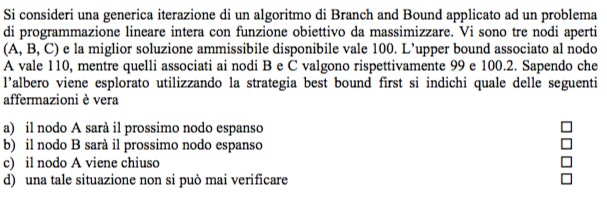
\includegraphics[width=\textwidth]{branch1}
  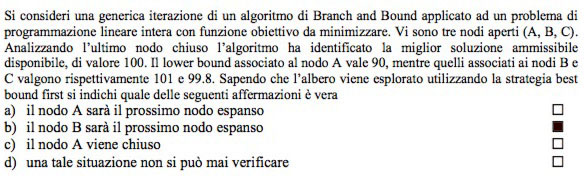
\includegraphics[width=\textwidth]{branch2}
  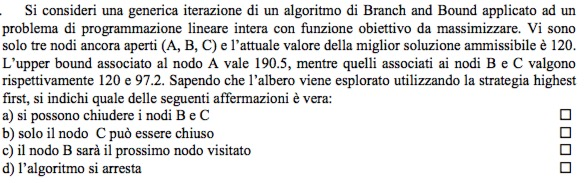
\includegraphics[width=\textwidth]{branch3}
\end{figure}
\subsection{Domande su problema duale}
\begin{figure}
  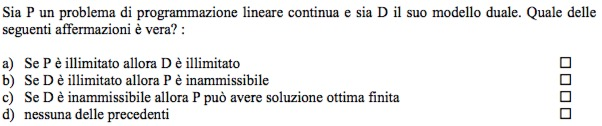
\includegraphics[width=\textwidth]{duale1}
  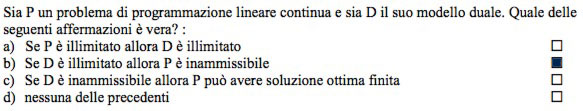
\includegraphics[width=\textwidth]{duale2}
  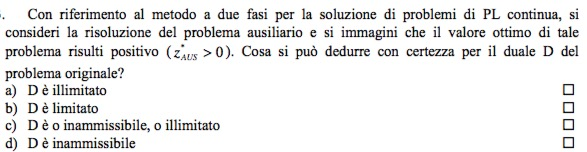
\includegraphics[width=\textwidth]{duale3}
\end{figure}
\subsection{Domande su rilassamento del problema lineare continuo}
\begin{figure}
  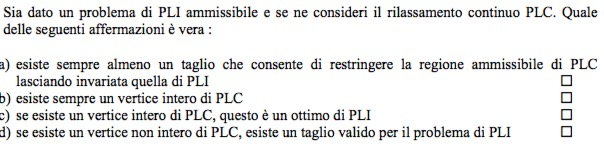
\includegraphics[width=\textwidth]{rilassamentoPLC1}
  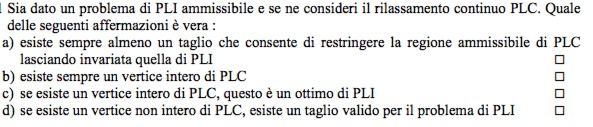
\includegraphics[width=\textwidth]{rilassamentoPLC2}
  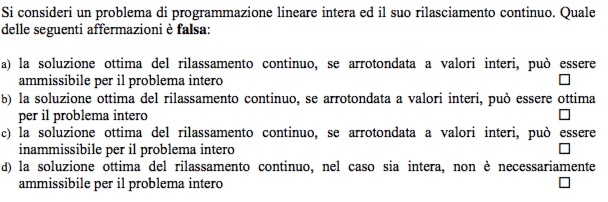
\includegraphics[width=\textwidth]{rilassamentoPLC3}
  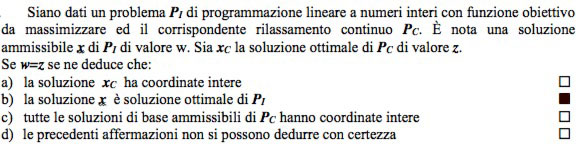
\includegraphics[width=\textwidth]{max3}
\end{figure}
\subsection{Domande su Analisi di sensitività}
\begin{figure}
  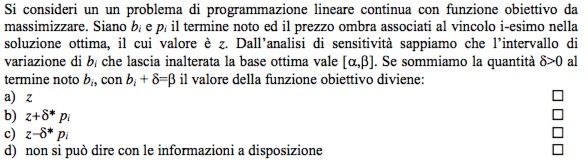
\includegraphics[width=\textwidth]{max2}
  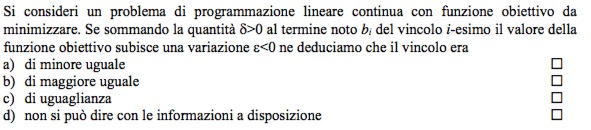
\includegraphics[width=\textwidth]{min1}
\end{figure}
\subsection{Domande varie}
\begin{figure}
  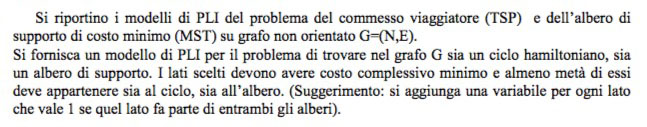
\includegraphics[width=\textwidth]{d6}
\end{figure}
\begin{figure}
  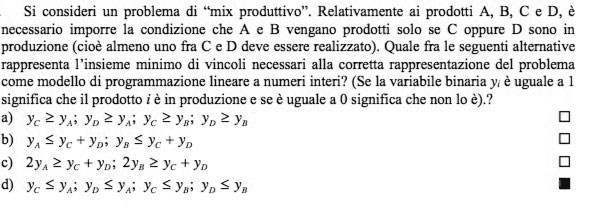
\includegraphics[width=\textwidth]{d7}
\end{figure}

\end{document}